% !TEX encoding = UTF-8 Unicode
% !TEX root = ../thesis.tex
\chapter{Introducción} \label{intro}
Este es un capítulo de ejemplo.

\section{Configuración de Página}

Los siguientes son los parámetros de configuración de la página de este formato. La Fig.~\ref{fig1_intro} muestra el formato que adopta \LaTeX\ para el Layout de la página. 

\pagevalues

\begin{figure}[ht]
	\pagediagram
	\caption{Diagrama de página}
	\label{fig1_intro}
\end{figure}

El tipo de letra es \textbf{Computer Modern Sans Serif}, con los tamaños que se indican en la Tabla~\ref{table2_intro}.

\begin{table}[htb]
\renewcommand{\arraystretch}{1.3}
	\caption{Tamaños de letra} 
	\label{table2_intro}
	\centering
	\setlength\tabcolsep{2pt}
	\begin{tabular}{c c}
		\hline
		\bfseries Sección & \bfseries Tamaño (pt)\\
		\hline
		 \bfseries Capítulo & 21  \\
		 \bfseries Sección & 15  \\
		 \bfseries Subsección & 12  \\
		 \bfseries Subsubsección & 11  \\
        \bfseries Texto / Encabezado& 11  \\
		\bfseries Pie de página & 9  \\
		\hline
	\end{tabular}
\end{table}

El encabezado de las páginas internas de capítulo se define de la siguiente manera: 
\begin{itemize}
    \item Páginas impares: Número y título de sección (izq), número de página (der)
    \item Páginas pares: Número de página (izq), número y título de capítulo (der)
\end{itemize}

Esto que sigue es un footnote: \footnote{footnote number 1 working fine}

Las referencias bibliográficas deben ser en estilo APA o IEEE. 

\section{Ejemplo de Tablas, Figuras y Ecuaciones}

Como se puede apreciar en la Fig.~\ref{fig2_intro}, los lápices tienen muchos colores, los mismos se pueden generar de diversas formas \cite{ejemplo}.

\begin{figure}[htb]
	\centering
	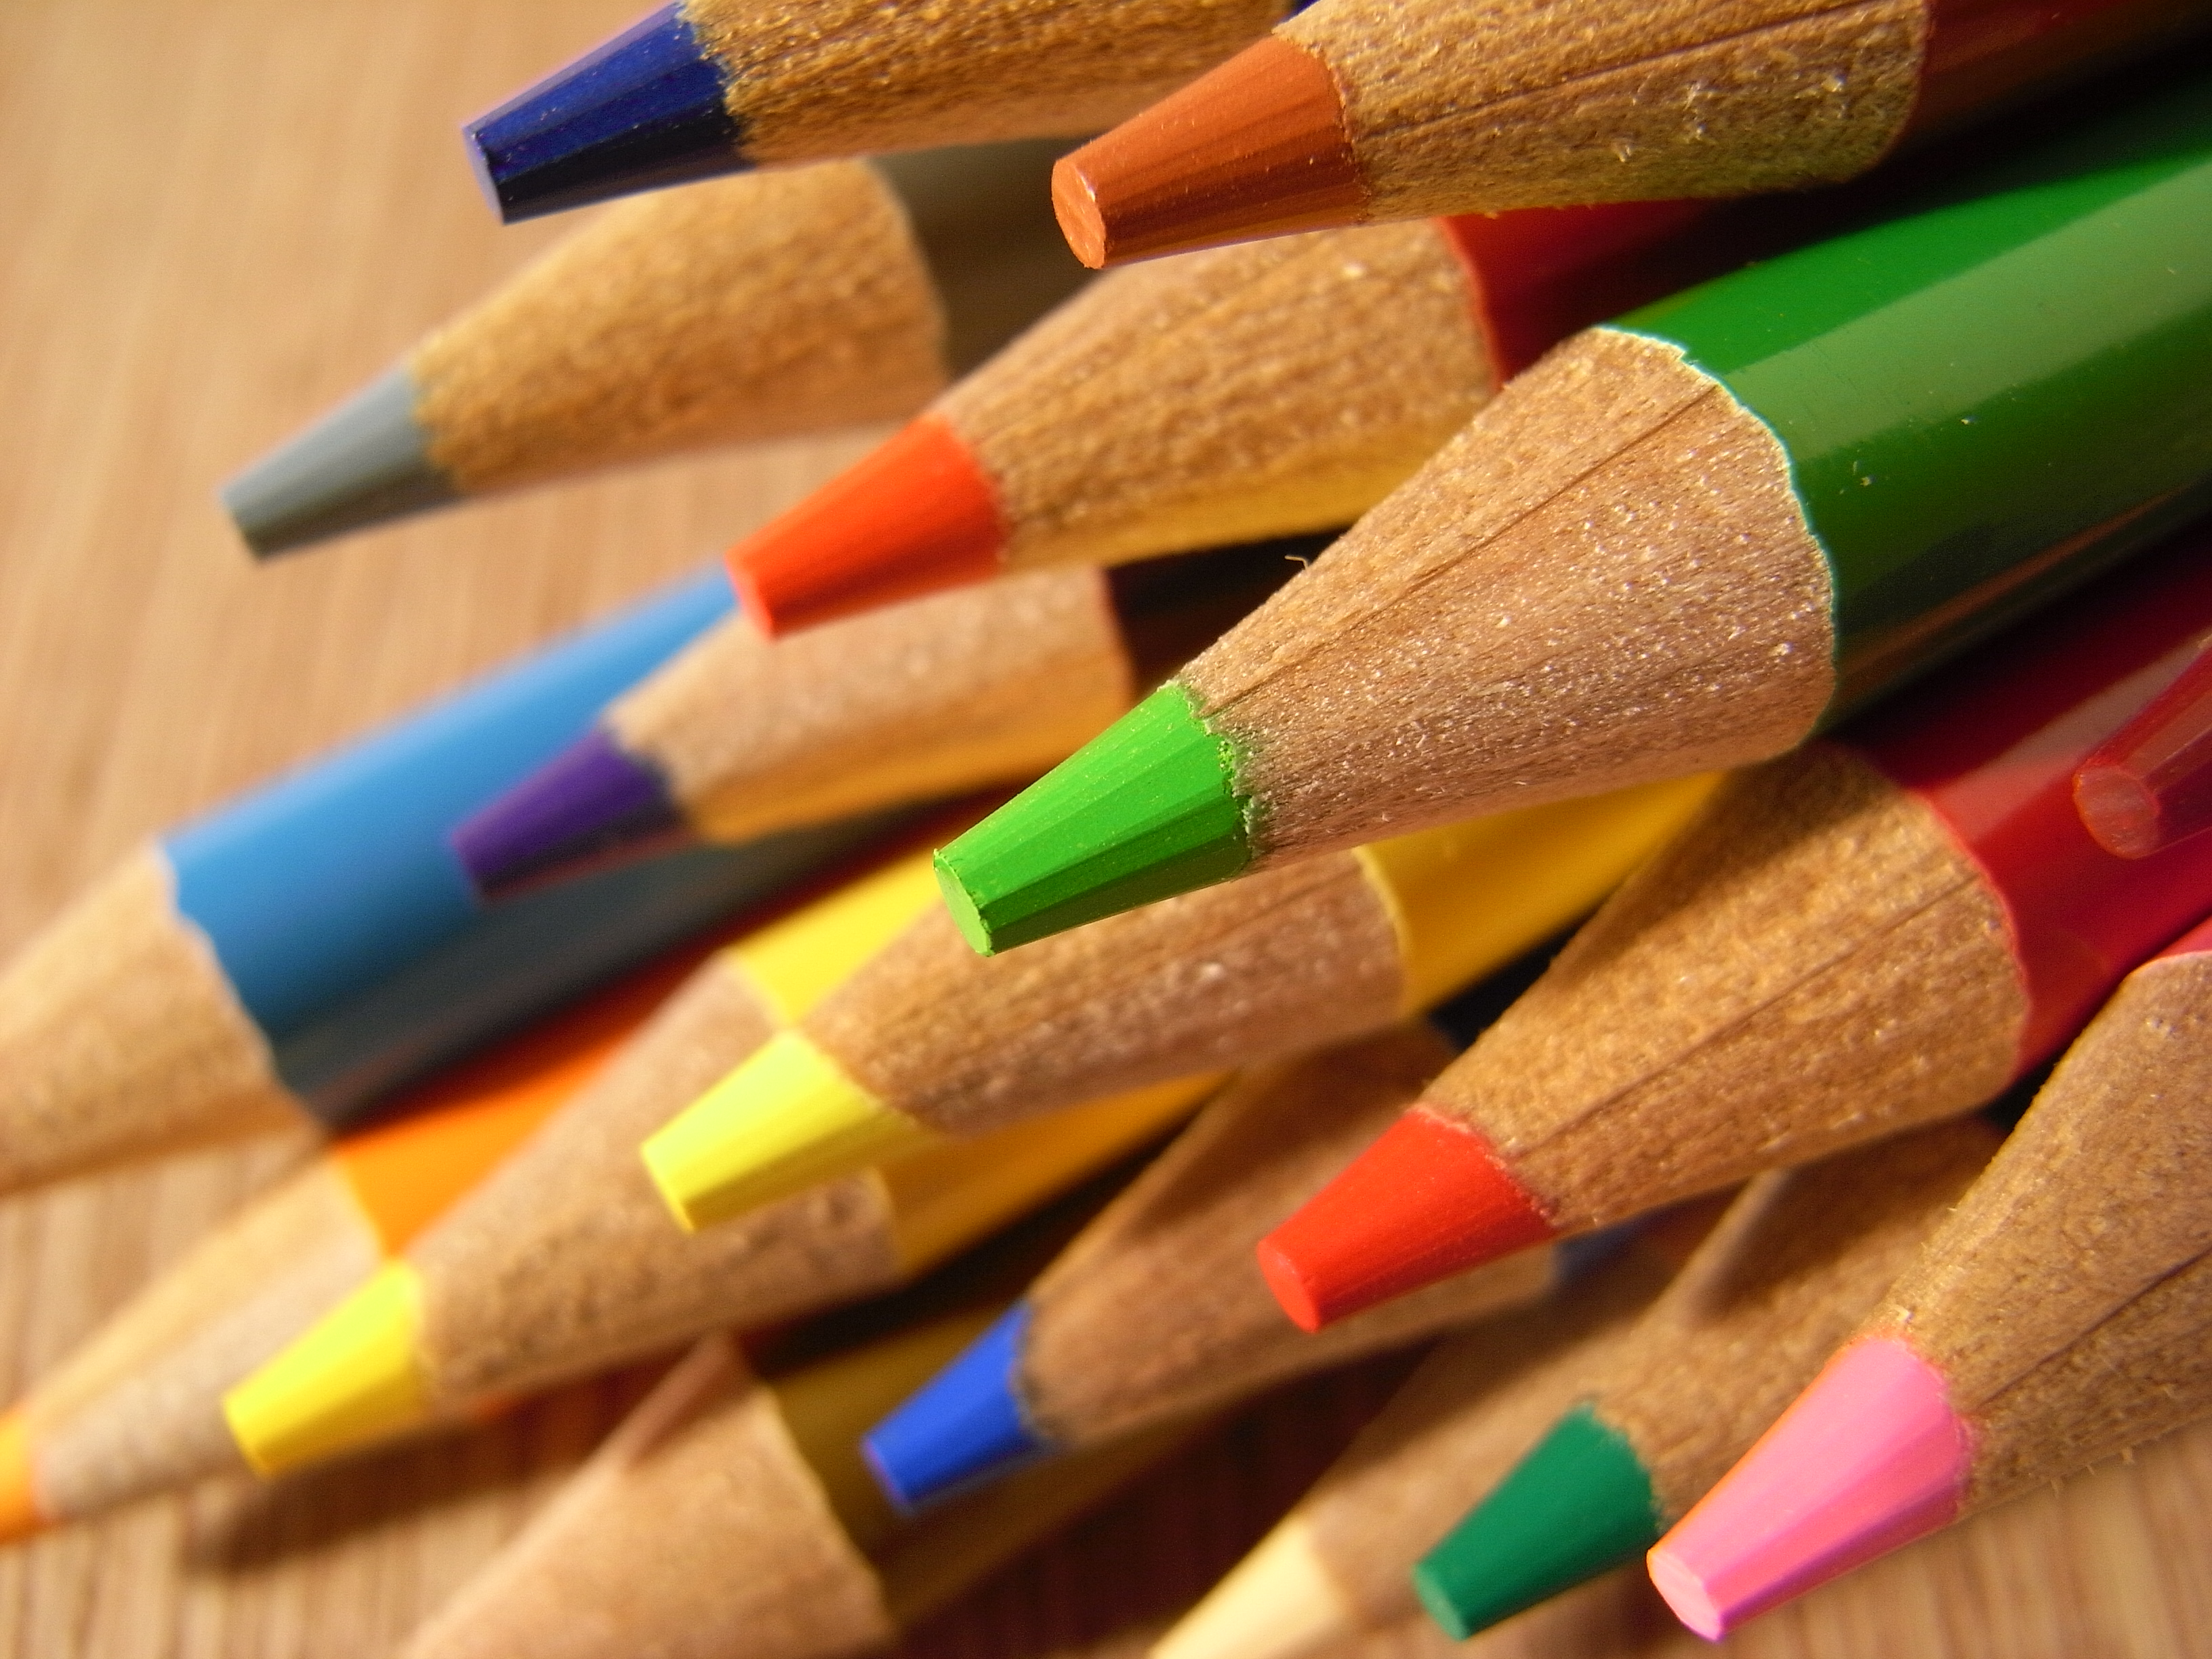
\includegraphics[width=0.8\textwidth]{figs/chapter1/sample.jpg} % width = 0.8\textwidth escala el ancho de la figura según el ancho del texto en la página
	\caption[Figura de ejemplo]{Figura de ejemplo, se incluye un texto lo suficientemente largo como para ver como queda distribuido en el documento}	% El que está entre corchetes va al ToC, el otro al documento
	\label{fig2_intro}
\end{figure}

En la Tabla~\ref{table1_intro} se observan los colores disponibles.
\begin{table}[htb]
\renewcommand{\arraystretch}{1.3}
	\caption[Colores]{Tabla de Colores} % Igual que el caption de la Figura. 
	\label{table1_intro}
	\centering
	\setlength\tabcolsep{2pt}
	\begin{tabular}{c c}
		\hline
		\bfseries Código & \bfseries Color\\
		\hline
		$\mathbf{v_1}$ & Rojo\\
		$\mathbf{v_2}$ & Azul\\
		$\mathbf{v_3}$ & Verde\\
		\hline
	\end{tabular}
\end{table}

Dada la ecuación de ejemplo:
\begin{equation}
	\label{eq1_chapter1}
	E=m\,c^2
\end{equation}
Si reemplazamos $m$ en \eqref{eq1_chapter1} obtenemos la energía. Esto que sigue es otro footnote: \footnote{footnote number 2 working fine}

\section{Escritura en Inglés}

Para quienes elijan escribir el documento en inglés, tener en cuenta las siguientes consideraciones: 
\begin{enumerate}
    \item Inmediatamente después de la carátula en castellano, agregue la carátula en inglés. 
    \item Al comienzo de cada capítulo, agregue un resumen en castellano de los contenidos del mismo, con una extensión máxima de dos páginas.
\end{enumerate}



